\documentclass[10pt]{book}
\usepackage[utf8]{inputenc}
\usepackage[italian]{babel}
\usepackage{multicol}
\usepackage[bookmarks]{hyperref}
\usepackage[a4paper, total={18cm, 25cm}]{geometry}
\usepackage{listings}
\usepackage{color}
\definecolor{gray}{rgb}{0.5,0.5,0.5}
\lstset{
	language=C,
	commentstyle=\itshape\color{gray},
	morekeywords={output}
}
\usepackage{graphicx}
\usepackage{makecell}
\graphicspath{ {./img/} }
\usepackage{color}

\begin{document}
\renewcommand*\contentsname{Indice}
\title{Crittografia}
\author{Federico Matteoni}
\date{A.A. 2020/21}
\maketitle
\tableofcontents
\pagebreak
\section*{Introduzione}
Prof.ssa: Anna Bernasconi.\\
Vedremo i cifrari da un punto di vista prettamente algoritmico. Vedremo anche i cifrari storici, ormai non più utilizzabili, perché hanno "aperto la strada", per poi passare ai cifrari perfetti (soluzione ideale ma con costo elevato).\\
Poi esamineremo i cifrari simmetrici, a chiave pubblica, curve ellittiche, firma digitale, SSL. Protocolli zero knowledge, blockchain e crittografia quantistica.\\\\
Libro di testo: Bernasconi, Ferragina, Luccio - Elementi di Crittografia.
\paragraph{Esame} Orali nel caso di esami a distanza, scritto nel caso di esami in presenza, closed-book.
\chapter{Introduzione alla Crittografia}
\section{Introduzione}
\paragraph{Crittografia} Significa "\textit{scrittura nascosta}", si intendono tecniche matematiche per mascherare i messaggi per non renderli leggibili a terzi (\textbf{crittografia}) o tentare di svelarli quando non si è il legittimo destinatario (\textbf{crittoanalisi}). Quindi tecniche di protezione e viceversa.\\
Esiste per i due mondi in contrapposizione: persone che vogliono scambiarsi privatamente informazioni e gli \textit{impiccioni} che desiderano ascoltare o intromettersi nelle conversazioni altrui (per curiosità, investigazione o altri scopi).
\paragraph{Due gruppi di persone} Chi vuole proteggersi userà \textbf{metodi di cifratura}, gli altri useranno \textbf{metodi di crittoanalisi}
\subparagraph{Crittografia} Metodi di Cifratura
\subparagraph{Crittoanalisi} Metodi di \ldots
\textbf{crittologia} studio comunicazione canali non sicuri e relativi problemi
\subsection{Lo scenario}
Alice vuole comunicare con Bob su un canale insicuro, quindi adottano un metodo di cifratura per spedire il messaggio in chiaro \texttt{m} sottoforma di crittogramma \texttt{c} (testo cifrato) che deve essere: incomprensibile al crittoanalista Eve (eavesdropper) in ascolto sul canale, ma facilmente decifrabile da Bob.
\paragraph{MSG} Insieme dei messaggi in chiaro
\paragraph{CRITTO} Insieme dei crittogrammi
\begin{center}
C : MSG $\rightarrow$ CRITTO\\
D : CRITTO $\rightarrow$ MSG
\end{center}
Sono operazioni da poter fare in tempo polinomiale. 
C e D sono una l'inversa dell'altra, ma C \textbf{deve essere iniettiva}.
\begin{center}
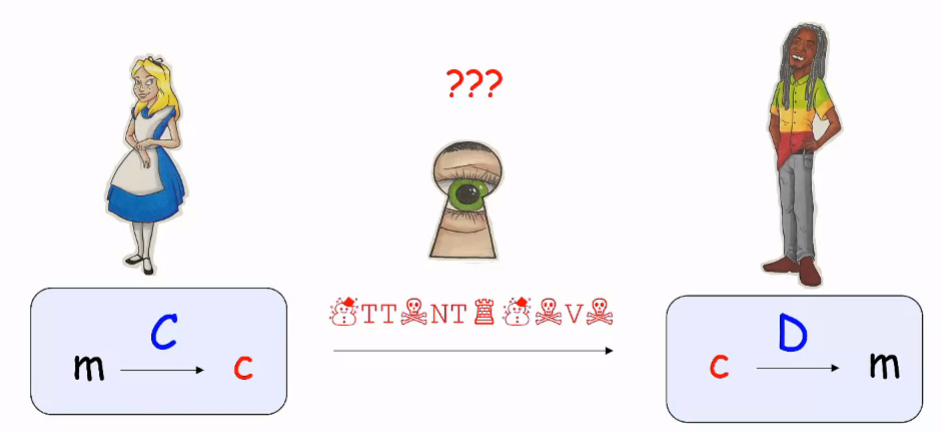
\includegraphics[scale=0.55]{1.png}
\end{center}
\subsection{Antichi esempi}
\paragraph{Erodoto} Nelle \textit{Storie}, V secolo a.C.\\
Messaggi tatuati sulla testa, coperti dai capelli e riscoperti rasando la testa.
\paragraph{Scitale} Spartani. Asta cilindrica in due esemplari identici. Si avvolgeva una striscia di carta attorno al cilindro e scritta. La chiave del cifrario è il diametro dello scitale.
\begin{center}
	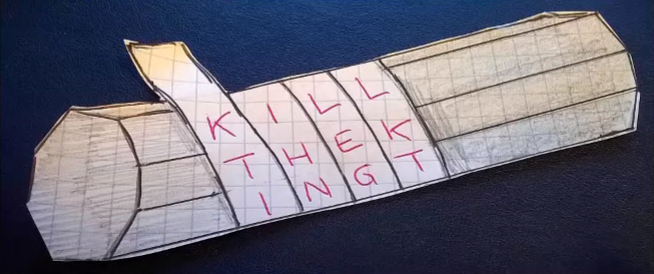
\includegraphics[scale=0.5]{2.png}
\end{center}
\paragraph{Enea Tattico} Un libro qualsiasi con un insieme di lettere segnate, o sostituire le vocali con simboli grafici.
\paragraph{Cifrario di Cesare} Il più antico cifrario di concezione moderna. L'idea di base è che il crittogramma è ottenuto dal messaggio in chiaro \texttt{m} sostituendo ogni lettera con quella di tre posizioni più avanti nell'alfabeto.\\
Es. A $\rightarrow$ D, Z $\rightarrow$ C. La segretezza dipende interamente dalla conoscenza del metodo, era destinato all'uso ristretto da un piccolo gruppo di persone.
\section{Livello di segretezza}
\paragraph{Classificazione} in base al livello di segretezza
\begin{list}{}{}
	\item Cifrari per \textbf{uso ristretto}\\
	Le tecniche con cui si calcola e decifra il crittogramma sono tenute segrete in ogni loro aspetto. Impiegati per comunicazioni classificate (diplomatiche o militari), non adatti per uso di massa.
	\item Cifrari per \textbf{uso generale}\\
	Ogni codice segreto non può essere mantenuto tale per troppo a lungo. La parte segreta si limita alla chiave, nota solamente agli utenti che stanno comunicando.\\
	Vengono studiati dalla comunità, coinvolgendo tantissime persone. Solo la chiave deve essere segreta.\\
	\textbf{Il nemico conosce il sistema}.\\
	Quindi C e D sono note, la chiave \textbf{segreta} \texttt{k} è usata come input sia in C che in D:\\
	\texttt{c = C(m, k)}, \texttt{m = D(c, k)}\\
	Se non si conosce \texttt{k}, anche conoscendo C e D non si possono estrarre informazioni dal crittogramma.\\
	Tenere segreta una sola chiave è più facile che segretare l'intero metodo. Tutti possono usare C e D pubbliche con chiavi diverse, e se un crittoanalista entra in possesso di una chiave posso generarne semplicemente una nuova.
\end{list}
\subsection{Chiavi segreta} Se la segretezza dipende unicamente dalla chiave bisogna proteggersi dagli attacchi a forza bruta, quindi avere un gran numero di chiavi, così da essere immuni da chi le prova tutte.\\
Inoltre la chiave deve essere scelta in modo casuale e non prevedibile, sennò il crittoanalista può provare le chiavi ovvie.
\paragraph{Attacco esauriente} Il crittoanalisa potrebbe sferrare un attacco a forza bruta verificando la significatività delle sequenze \texttt{D(c, k)} $\forall$ \texttt{k}.\\
Se $|$Key$|$ = $10^{20}$ e con un calcolatore che impiega $10^{-6}$ per calcolare \texttt{D(c, k)} servirebbe in media più di un milione di anni per scoprire il messaggi provando tutte le chiavi. Però la segretezza può essere violata con altre tecniche: esistono cifrari più sicuri di altri pur con uno spazio di chiavi più piccoli.\\
Un cifrario complicato non è necessariamente più sicuro e \textbf{mai sottovalutare la bravura del crittoanalista}.
\subsection{Crittoanalista}
\paragraph{Comportamento} Il comportamento di un crittoanalista può essere:
\begin{list}{}{}
	\item \textbf{Passivo}, quando si \textbf{limita ad ascoltare} la comunicazione
	\item \textbf{Attivo}, quando \textbf{agisce sul canale} disturbando la comunicazione o modificando il contenuto dei messaggi.
\end{list}
\paragraph{Attacchi a un sistema crittografico} Hanno l'obiettivo di forzare un sistema. Il metodo e il livello di pericolosità dipendono dalle informazioni in possesso del crittoanalista:
\begin{list}{}{}
	\item \textbf{Cipher Text Attack}: conosce una serie di crittogrammi
	\item \textbf{Known Plain-Text Attack}: conosce una serie di coppie \texttt{(m, c)}
	\item \textbf{Chosen Plain-Text Attack}: si procura coppie \texttt{(m, c)} relative a messaggi in chiaro da lui scelti.\\
	Tutta la crittografia a chiave pubblica è soggetta a questo tipo di attacco (avendo la chiave pubblica, cifro dei messaggi che penso possano passare e ascolto finché non trovo nella comunicazione i crittogrammi in mio possesso).
\end{list}
\paragraph{Man in the Middle} Il crittoanalista si installa sul canale di comunicazione:
\begin{list}{}{}
	\item \textbf{Interrompe le comunicazioni dirette} tra gli utenti Alice e Bob
	\item le \textbf{sostituisce con messaggi propri}
	\item e \textbf{convince} ciascun utente \textbf{che tali messaggi provengano leggitimamente dall'altro} utente.
\end{list}
Quindi il crittoanalista \textbf{Eve si finge Bob agli occhi di Alice e Alice agli occhi di Bob}.
\paragraph{Esiti}
\begin{list}{}{}
	\item Successo pieno, si scopre completamente D o si ottiene la chiave
	\item Successo limitato, si scopre solo qualche informazione ma sufficiente per comprendere il messaggio
\end{list}
\subsection{Situazione attuale}
\paragraph{Cifrari perfetti} Inattaccabili, esistono ma richiedono operazioni complesse, \textbf{chiavi lunghe tanto quanto il messaggio e mai riutilizzabili}.\\
\textbf{Shannon}, 1945 (pubblicato nel 1949 per motivi di segretezza militare): \texttt{m} e \texttt{c} appaiono totalmente scorrelati, come se \texttt{c} fosse una stringa casuale di bit.\\Nessuna informazione può filtrare dal crittogramma. Vedremo la teoria matematica.
\subparagraph{One-Time Pad} Anche detto blocco monouso, sicuro ma per essere usato bene richiede chiavi segrete totalmente casuali e lunghe quanto il messaggio. Come generarla e come scambiarla?
\paragraph{Cifrari attuali} Nella crittografia di massa non si usano cifrari perfetti, ma \textbf{cifrari \textit{dichiarati} sicuri}, inviolati dagli esperti e che usano algoritmi solo esponenziali per decrittare senza chiave. Il tempo per violare un cifrario è enorme e rende l'operazione insostenibile $\rightarrow$ impossibilità \textit{pratica} di forzare il cifrario.
\subparagraph{Dichiarati sicuri} Non è noto se questi problemi matematici richiedano algoritmi \textit{necessariamente} esponenziali o se sono dovuti all'incapacità nostra di trovare metodi più efficienti. Si riconduce a $P = NP$
\subsection{Cifrari odierni}
\paragraph{Advanced Encryption Standard} AES, simmetrico a blocchi con chiavi di 128-256bit, pubblicamente noto e realizzabile su computer di ogni tipo. Il messaggio è diviso a blocchi lunghi quanto la chiave.
\paragraph{Le chiavi} Sono stabilite dai mezzi elettronici (PC, smartphone, terminale...) e su Internet si scambia una chiave per ogni sessione.
\subparagraph{Scambio delle chiavi} La chiave va comunicata in sicurezza su un canale non ancora sicuro. Un'intercettazione nello scambio della chiave compromette il sistema.\\
Nel 1976 viene proposto un algoritmo per generare e scambiare una chiave segreta su un canale insicuro, senza necessità di scambiare informazioni o di incontrarsi in precedenza.\\
Si chiama \textbf{protocollo DH}, ancora largamente utilizzato nei protocolli crittografici su Internet.\\
Si scambiano pezzi di chiave tramite la rete e unendole a informazioni locali si costruisce la chiave.
\subparagraph{Chiave pubblica} Diffie ed Hellman hanno anche proposto la crittografia a chiave pubblica.
\begin{list}{}{}
	\item \textbf{Cifrari simmetrici}: stessa chiave per cifrare e decifrare, nota solo ai due utenti che comunicano. La scelgono di comune accordo e la tengono segreta.
	\item \textbf{Cifrari asimmetrici}: chiavi pubbliche usate per cifrare e chiavi private per decifrare.\\
	\texttt{c = C(m, k$_{pub}$)}\\
	\texttt{m = D(m, k$_{prv}$)}\\
	Si rende necessario che la C sia una one-way trapdoor: calcolare il crittogramma deve essere facile (polinomiale), ma decifrare \texttt{c} deve essere computazionalmente difficile (a meno di conoscere la trapdoor, la chiave privata).
\end{list}
\paragraph{RSA} Rivest, Shamir, Adleman, 1977. Propongono un sistema a chiave pubblico facile da calcolare e difficile da invertire.
\paragraph{Vantaggi}
\begin{list}{}{}
	\item Comunicazione molti a uno\\
	Tutti possono inviare in modo sicuro allo stesso destinatario usando la sua chiave pubblica, ma solo lui può decifrarli. Un crittoanalista non può decifrare anche se conosce C, D e k$_{pub}$
	\item Se $n$ utenti vogliono comunicare servono solo $2n$ chiavi invece delle $n(n-1)/2$ necessarie nei cifrari simmetrici (una coppia per ogni coppia di utenti)
	\item Non è richiesto nessun scambio
\end{list}
\paragraph{Svantaggi}
\begin{list}{}{}
	\item Sono molto lenti rispetto ai cifrari simmetrici (polinomi di terzo grado)
	\item Sono esposti ad attacchi di tipo chosen plain-text, perché conosco la chiave pubblica\\
	Scelgo un numero qualsiasi di messaggi in chiaro, costruisce i crittogrammi relativi e ascolta sul canale confrontando i crittogrammi in transito e se trova un riscontro sa esattamente qual è il messaggio passato.
\end{list}
\paragraph{Come si usa} Oggi si usa un cifrario a chiave segreta (AES) per le comunicazioni di massa, e un cifrario a chiave pubblica per scambiare le chiavi segrete relative al primo senza incontri fisici tra gli utenti.\\
Diventa lento solo lo scambio delle chiavi. Siamo anche al sicuro da attacchi chosen plain-text perché se la chiave è scelta bene risulta imprevedibile dal crittoanalista.
\section{Rappresentazione matematica di oggetti}
Per rappresentare gli oggetti scegliamo dei \textbf{caratteri} da un \textbf{insieme finito} detto \textbf{alfabeto}.\\
Un \textbf{oggetto} è \textbf{rappresentato da una sequenza ordinata di caratteri dell'alfabeto}. L'ordine dei caratteri è importante: a \textbf{oggetti diversi corrispondono sequenze diverse} e \textbf{il numero di oggetti che si possono rappresentare non ha limiti}. Significa che fissando un numero $n$ arbitrariamente grande possiamo sempre creare un numero di oggetti $> n$, con sequenze via via più grande.
\paragraph{Alfabeto} $\Gamma$ con $|\Gamma| = s$ e $N$ oggetti da rappresentare.\\
$d(s, N)$: lunghezza della sequenza più lunga che rappresenta un oggetto dell'insieme. A noi interessa la rappresentazione che minimizza $d(s, N)$, cioè $d_{min}(s, N)$\\
Una rappresentazione è tanto più efficiente quanto $d(s, N)$ si avvicina a $d_{min}(s, N)$
\paragraph{Esempio} $s = 1, \Gamma = \{0\}$ l'unica possibilità è variare la lunghezza $\Rightarrow d_{min}(1, N) = N$, estremamente sfavorevole.\\
$s = 2, \Gamma = \{0, 1\}$, $\forall\:k\geq 1$ ho $2^k$ sequenze di lunghezza $k$. Il numero totale di sequenze lunghe da $1$ a $k$ è $2^{k+1} - 2$ (si esclude anche la sequenza nulla). Con $N$ oggetti da rappresentare $\Rightarrow k \geq \log_2(N+2) - 1 \Rightarrow N$ sequenze diverse tutte di $\log_2(N)$ caratteri.
\paragraph{Efficiente} Codifica efficiente quando c'è questa riduzione logaritmica, \textbf{efficiente} quando \textbf{}. Sequenze della stessa lunghezza è vantaggioso perché non servono caratteri separatori. Per questo è necessario che l'alfabeto contenga almeno due caratteri.\\
La \textbf{notazione posizionale} è una rappresentazione efficiente indipendentemente dalla base $s \geq 2$ scelta. Un intero $N$ è rappresentato con un numero $d$ di cifre $|\: \log_s(N) \leq d \leq \log_s(N) + 1$
\section{Richiamo della teoria della calcolabilità}
\paragraph{Problemi computazionali} Formulati matematicamente di cui cerchiamo una soluzione algoritmica: \textbf{decidibili} (e \textbf{trattabili} o \textbf{non trattabili}), o \textbf{non decidibili}.\\
Calcolabilità $\rightarrow$ \textbf{Algoritmo} e \textbf{problema non decidibile}\\
Complessità $\rightarrow$ \textbf{Algoritmo efficiente} e \textbf{problema intrattabile}.
\paragraph{Numerabilità} Due insiemi $A$ e $B$ hanno lo stesso numero di elementi $\Leftrightarrow$ si può stabilire una \textbf{corrispondenza biunivoca} tra i loro elementi.\\
Questo porta alla definizione di \textbf{numerabile}: un insieme è numerabile $\Leftrightarrow$ i suoi elementi possono essere messi in \textbf{corrispondenza biunivoca con i numeri naturali}.\\
Numerabile significa che \textbf{possiede un'infinità numerabile di elementi}. Esempi: l'insieme dei numeri naturali $N$, l'insieme degli interi $Z$ (avendo $n$ in corrispondenza biunivoca con $2n + 1$ per $n\geq 0$ e $n \leftrightarrow 2|n|$ per $n < 0$, dando la sequenza $0, -1, 1, -2, 2\ldots$) o anche l'insieme dei naturali pari ($2n \leftrightarrow n$)
\paragraph{Enumerazione delle sequenze} Si vuole elencare in uno ordine ragionevole le sequenze di lunghezza finita costruite su un alfabeto finito. Le sequenze non sono in numero finito, quindi non si potrà completare l'elenco.\\
Lo scopo è \textbf{raggiungere qualsiasi sequenza $\sigma$ arbitrariamente scelta in un numero finito di passi}. $\sigma$ deve dunque trovarsi a \textbf{distanza finita} dall'inizio dell'elenco. Non va bene l'ordine del dizionario perché non saprei la posizione della prima stringa che inizia con $b$ perché le stringhe composte da tutte $a$ sono infinite.\\
Si stabilisce un ordine tra i caratteri. Si ordinano prima in lunghezza crescente e, a pari lunghezza, in ordine alfabetico.
\paragraph{Esempio} $\Gamma = \{a, b, \ldots, z\}$, avrei\\
$a, b, \ldots, z,$\\
$aa, ab, \ldots, az, ba, bb, \ldots, bz, \ldots, zz,$\ldots\\
Ad una sequenza arbitraria corrisponde un numero intero, e la sequenza $s$ arbitraria si troverà tra quelle di lunghezza $|s|$ in posizione alfabetica. Quindi ad una sequenza arbitraria $\leftrightarrow$ $n$ che indica la posizione nell'elenco, e ad un numero naturale $n \leftrightarrow$ la sequenza che occupa l'$n$-esima posizione nell'elenco.\\\\
La \textbf{numerazione delle sequenze è fattibile perché sono di lunghezza finita}, anche se illimitata. Cioè per qualunque intero $d$ scelto a priori, esistono sequenze di lunghezza maggiore di $d$. Per sequenze di lunghezza infinita la numerazione non è possibile
\paragraph{Insiemi non numerabili} Insiemi non equivalenti a $N$ come $R$, $(0, 1)$, l'insieme di tutte le linee del piano, insieme delle funzioni in una o più variabili\ldots $\Rightarrow$ l'\textbf{insieme dei problemi computazionali non è numerabile}. Perché un problema computazionale è sempre visualizzabile come una funziona matematica, che associa ad ogni insieme di dati espressi da $k$ numeri interi il corrispondente risultato espresso da $j$ numeri interi $$f:N^k \rightarrow N^j$$
Quindi l'insieme di queste $f$ \textbf{non è numerabile}.
\paragraph{Diagonalizzazione}
$F = \{$ funzioni $f\:|\: f: N \rightarrow \{0, 1\}\}$, ogni $f\in F$ è rappresentata da una sequenza infinita
\begin{list}{}{}
	\item $x$ 0 1 2 3 \ldots n \ldots
	\item $f(x)$ 0 1 0 1 \ldots 0 \ldots
\end{list}
ma se è possibile è rappresentabile con una regola (f 0 se x pari 1 se x dispari)\\
Per assurdo, ipotizzo F numerabile. Si può assegnare ad ogni funzione un numero progressivo nella numerazione e costruire una tabella infinita con tutte le funzioni.
\begin{center}
	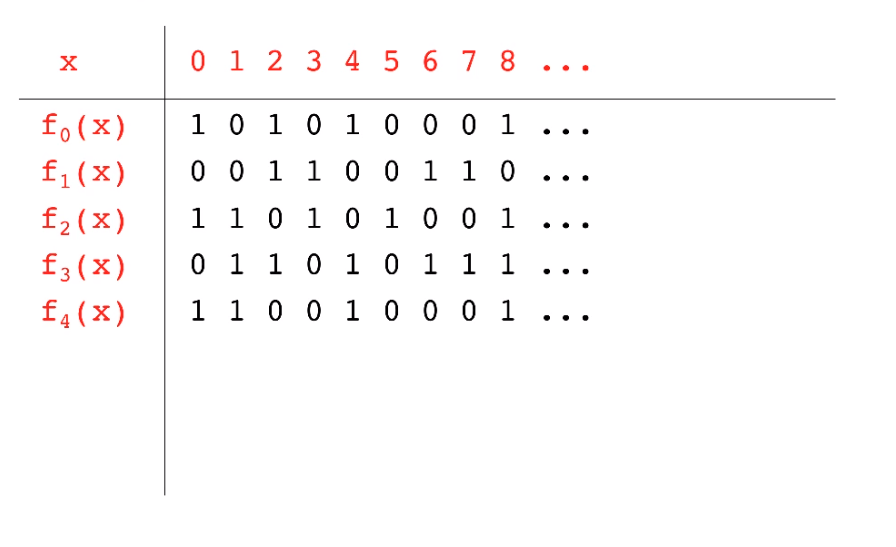
\includegraphics[scale=0.6]{3.png}
\end{center}
Definisco $g(x)$ = $\left\{ \begin{array}{l l}
0 & f_x(x) = 1\\ 1 & f_x(x) = 0
\end{array} \right. \Rightarrow g$ non può corrispondere a nessuna delle $f_i$ della tabella, perché differisce da tutte le funzioni almeno nella diagonale principale.\\
$g(x)\:\:|\:\:\:0\:1\:1\:1\ldots$\\
Per assurdo $\exists\:j\:|\:g(x) = f_j(x) \Rightarrow g(j) = f_j(j)$ ma per la definizione $g(j)$ è il complemento di $f_j(j)$, quindi $g(j) \neq f_j(j)$ \textbf{contraddizione}.\\
Per qualunque numerazione scelta esiste sempre almeno una funzione esclusa, quindi $F$ non è numerabile.
\subsection{Algoritmi}
\paragraph{Algoritmi} la \textbf{formulazione di un algoritmo}, una sequenza finita di operazioni, completamente e univocamente determinate, \textbf{dipende dal modello di calcolo utilizzato}.\\
Qualunque modello si scelga, gli algoritmi devono essere descritti da sequenze finite di caratteri di un alfabeto finito $\Rightarrow$ sono \textbf{possibilmente infiniti ma numerabili}.
\paragraph{Problemi computazionali} Sono \textbf{funzioni matematiche} che associano ad ogni insieme di dati il corrispondente risultato, e \textbf{non sono numerabili} come visto prima.
\paragraph{Problema della rappresentazione} C'è una drastica perdita di potenza, perché gli algoritmi sono numerabili ma sono meno dei problemi computazionali $$|\{Problemi\}| >> |\{Algoritmi\}|$$
$\Rightarrow$ \textbf{esistono problemi privi di un corrispondente algoritmo di calcolo}. Per esempio, il problema dell'arresto.
\paragraph{Lezione di Turing} \textit{Non esistono algoritmi che decidono il comportamento di altri algoritmi esaminandoli dall'esterno, cioè senza passare dalla loro simulazione}.
\subsection{Modelli di calcolo}\begin{center}
La teoria della calcolabilità dipende dal modello di calcolo?\\
Oppure\\
la decidibilità è una proprietà del problema?
\end{center}
\pagebreak
I linguaggi di programmazione esistenti sono tutti equivalenti?\\
Ce ne sono di alcuni più potenti/più semplici di altri?\\
Ci sono algoritmi descrivibili in un linguaggio ma non in un altro?\\
È possibile che problemi oggi irrisolvibili possano essere risolti in futuro con altri linguaggi o altri calcolatori?\\
Le teorie della calcolabilità e della complessità dipendono dal modello di calcolo?
\paragraph{Tesi di Church-Turing} Tutti i \textit{ragionevoli} modelli di calcolo \textbf{risolvono esattamente la stessa classe di problemi}, quindi \textbf{si equivalgono nella possibilità di risolvere i problemi} pur operando con diversa efficienza.
\begin{center}
\textbf{Tesi C-H: la decidibilità è una proprietà del problema}
\end{center}
Incrementi qualitativi sui calcolatori o sui linguaggi di programmazione servono \textbf{solo} ad abbassare i tempi di esecuzione o rendere più agevole la programmazione.
\subsection{Decidibilità e trattabilità}
Ci sono quindi problemi che non possono essere risolti da nessun calcolatore, indipendentemente dal tempo impiegato (\textbf{problemi indecidibili}).\\
Ci sono poi problemi decidibili che possono richiedere tempi di risoluzione esponenziali nella dimensione dell'istanza (\textbf{problemi intrattabili}).\\
Ci sono poi problemi che possono essere risolti con algoritmi di costo polinomiale nella dimensione dell'inpu\\(\textbf{problemi trattabili}).\\
Abbiamo poi una famiglia di problemi il cui stato non è noto: clique (cricca), cammino hamiltoniano\ldots Sappiamo risolverli (decidibili) con algoritmi di costo esponenziale, ma non abbiamo limiti inferiori esponenziali. I migliori limiti inferiori sono polinomiali: c'è un gap fra il limite inferiore (polinomiale) e costo della migliore soluzione a disposizione (esponenziale) (\textbf{presumibilmente intrattabili}).
\subsubsection{Notazione}
Studiamo la dimensione dei dati trattabili in funzione dell'incremento della velocità del calcolatori.\\
Dati i calcolatori $C_1$, $C_2$ ($k$ volte più veloce di $C_1$) e tempo di calcolo a disposizione $t$, avrò $n_1$ dati trattabili in tempo $t$ su $C_1$ e $n_2$ trattabili in tempo $t$ su $C_2$.\\\\
Si \textbf{osserva} che \textbf{usare $C_2$ per un tempo $t$ equivale a usare $C_1$ per un tempo $k\cdot t$}.
\paragraph{Algoritmi polinomiali} Un algoritmo polinomiale che risolve il problema in $c\cdot n^s$ secondi, con $c$ ed $s$ costanti.
\begin{list}{}{}
	\item[$C_1$] $c\cdot n_1^s = t \Rightarrow n_1 = (t/c)^{1/s}$
	\item[$C_2$] $c\cdot n_2^s = t \Rightarrow n_2 = k^{1/s}\cdot(t/c)^{1/s}$
	\item[$\Rightarrow$] $n_2 = k^{1/s}\cdot n_1$, miglioramento di un fattore \textbf{moltiplicativo} $k^{1/s}$
\end{list}
\paragraph{Algoritmi esponenziali} Un algoritmo polinomiale che risolve il problema in $c\cdot 2^n$ secondi, con $c$ costante.
\begin{list}{}{}
	\item[$C_1$] $c2^{n_1} = t \Rightarrow 2^{n_1} = t/c$
	\item[$C_2$] $c2^{n_2} = k\cdot t \Rightarrow 2^{n_1} = k\cdot t/c = k2^{n_1}$
	\item[$\Rightarrow$] $n_2 = n_1 + \log_2(k)$, miglioramento di un fattore \textbf{additivo} $\log_2(k)$
\end{list}
Di conseguenza \textbf{un algoritmo efficiente è di gran lunga più importante di un calcolatore più potente}.
\subsection{Tipologie di problemi}
Dato un problema $\Pi$ su un insieme di istanze in ingresso $I$ con un insieme di soluzioni $S$.
\paragraph{Problemi decisionali} Richiedono una risposta binaria $S=\{0, 1\}$, quindi istanze positive $x\in I\:|\:\Pi(x) = 1$ o negative $x\in I\:|\:\Pi(x) = 0$. Esempio: verifica se un numero è primo, o se un grafo è connesso.\\
La teoria della complessità computazionale è definita principalmente in termini di problemi di decisione: risposta binaria, quindi il tempo per restituire la risposta è costante, e la complessità di un problema è già presente nella versione decisionale.
\paragraph{Problemi di ricerca} Data un'istanza $x$, richiede di restituire una soluzione $s$.
\paragraph{Problemi di ottimizzazione} Data un'istanza $x$, si vuole trovare la \textbf{migliore} soluzione $s$ tra tutte quelle possibili. Esempio: clique di dimensione massima, cammino minimo\ldots
\subsection{Classi di complessità}
Dato un problema \textbf{decisionale} $\Pi$ ed un algoritmo $A$, diciamo che \textbf{$A$ risolve $\Pi$} se, data un'istanza di input $x$, $A(x) = 1 \Leftrightarrow \Pi(x) = 1$\\
$A$ risolve $\Pi$ in \textbf{tempo $t(n)$ e spazio $s(n)$}.
\paragraph{Classi Time e Space}
\begin{list}{}{}
	\item Time($f(n)$): insieme dei \textbf{problemi decisionali che possono essere risolti in tempo O($f(n)$)}
	\item Space($f(n)$): insieme dei \textbf{problemi decisionali che possono essere risolti in spazio O($f(n)$)}
\end{list}
\paragraph{Classe P} Classe dei problemi risolvibili in \textbf{tempo} polinomiale nella dimensione dell'istanza di input.\\
\textbf{Algoritmo polinomiale} nel tempo: $\exists\:c, n_0 > 0\:\:|\:\:$ il numero di passi elementari è al più $n^c$ per ogni input di dimensione $n > n_0$.
\paragraph{Classe PSPACE} Classe dei problemi risolvibili in \textbf{spazio} polinomiale nella dimensione dell'istanza di input. Molto più grande di P.\\
\textbf{Algoritmo polinomiale} nello spazio: $\exists\:c, n_0 > 0\:\:|\:\:$ il numero di celle di memoria è al più $n^c$ per ogni input di dimensione $n > n_0$.
\paragraph{Classe EXPTIME} Classe dei problemi risolvibili in tempo esponenziale nella dimensione dell'istanza di input.
$$P\subseteq PSPACE \subseteq EXPTIME$$
Non è noto se queste inclusioni siano note, ad oggi. L'unico risultato dimostrato finora riguarda P ed EXPTIME: esiste un problema che può essere risolto in tempo esponenziale ma per cui il tempo polinomiale non è sufficiente (es: torri di Hanoi).
\subsection{Certificato}
Per alcuni problemi, per le istanze accettabili (istanze in cui la risposta del problema decisionale è si), è possibile certificare che quell'istanza è accettabile con un certificato $y$ che può convincerci dell'accettabilità.\\
Per clique, il certificato è il sottoinsieme di $k$ vertici che forma la clique. Per il cammino hamiltoniano è la permutazione degli $n$ vertici che formano il cammino. Per SAT, sono le assegnazioni che rendono vera la formula. Il certificato ha dimensione polinomiale ($k, n$) e la verifica del certificato è lineare.\\
Una volta che ho il certificato lo vado a verificare: attestato breve di esistenza di una soluzione con determinate proprietà. Si definisce solo per istanze accettabili, perché spesso la non accettabilità non è facile costruire un certificato.
\paragraph{Idea} Usare il costo della verifica di un certificato per un'istanza accettabile per \textbf{caratterizzare la complessità del problema} stesso.\\
Un problema è \textbf{verificabile in tempo polinomiale} se: tutte le istanze accettabili ammettono un certificato di lunghezza polinomiale ed esiste un algoritmo di verifica polinomiale in n.
\paragraph{Classe NP} Classe dei problemi decisionali \textbf{verificabili in tempo polinomiale}. (NP = polinomiale su macchine non deterministiche)
\paragraph{P $\subset$ NP?} Ovviamente si, ogni problema in P ammette un certificato verificabile in tempo polinomiale: eseguo l'algoritmo che risolve il problema per costruire il certificato.\\
Quello che non sappiamo è $P = NP$ oppure $P \neq NP$. Si pensa $P \neq NP$.\\
Si possono individuare i problemi più difficili in NP, ovvero quelli candidati ad appartenere ad NP se $P \neq NP$: sono i problemi NP-completi, quelli per cui se esiste un algoritmo polinomiale per risolvere un NP-completo allora tutti i problemi NP potrebbero essere risolti in tempo polinomiale e quindi P = NP.\\
Quindi tutti i problemi NP-completi sono risolvibili in tempo polinomiale oppure nessuno lo è.\\\\
Tutti i problemi NP-completi possono essere ridotti l'un l'altro, sono NP-equivalenti.
\paragraph{Gerarchia delle classi secondo le attuali congetture}
\begin{center}
	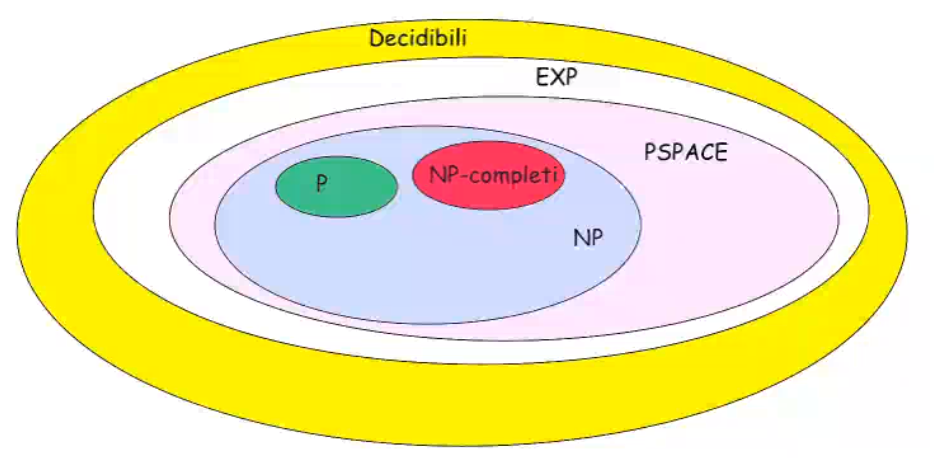
\includegraphics[scale=0.75]{4.png}
\end{center}
La fattorizzazione ad esempio $\in NP - (P \cup NPcompleti)$, infatti è risolto in tempo polinomiale su macchine quantistiche.
\subsection{Classi co-P e co-NP}
C'è molta differenza tra certificare l'esistenza e certificare la non esistenza di una soluzione. Dato un problema $\Pi$ possiamo definire co$\Pi$ che accetta tutte e sole le istanze rifiutate da $\Pi$.\\
La classe coP è la classe per cui co$\Pi\in$ P. P = coP, i problemi complementari e i co-complementari (originali) si possono entrambi risolvere in tempo polinomiale: risolvo il problema complementare e complemento il risultato.\\\\
Questo non vale per coNP, la classe per cui co$\Pi\in$ NP. Si congettura che siano diverse, se la congettura è vera allora $P\neq NP$
\begin{center}
	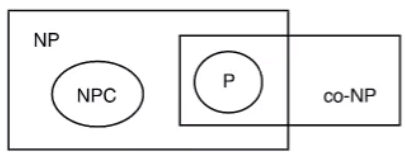
\includegraphics[scale=0.5]{5.png}
\end{center}
\chapter{Sequenze Casuali}
\section{Esempi di algoritmi numerici}
\paragraph{Algoritmo di Euclide} Algoritmo per il calcolo dell'MCD fra due interi.\\
Suppongo due interi $a$, $b$ con $a \geq b$, $a > 0$ e  $b \geq 0$\\
MCD$(a,b) = \left\{ \begin{array}{l l}
a & b = 0\\
MCD(a, a\: mod\: b) & else
\end{array}\right.$
\subparagraph{Valutazione complessità} Data I istanza di input composta da $a$, $b$, vengono rappresentati ad esempio in base due. Quindi la dimensione $n$ dell'istanza di input I $n = \:|I|\:=\Theta(\log a + \log b) = \Theta(\log a)$.\\
L'algoritmo è ricorsivo, quindi bisogna valutare il numero delle chiamate ricorsive, che dipenderanno dai dati. Ci saranno istanze in cui si termina subito (ad esempio se $a$ multiplo di $b$, cioè $a$ mod $b = 0$). In generale, \textbf{il numero di chiamate cresce con $\log a$}, perché $a$ mod $b$ rimpiazza $a$.\\\\
Si osserva che $a$ mod $b < \frac{a}{2}$\\
Questo perché $a = qb + (a$ mod $b)$ e siccome per ipotesi $a \geq b \Rightarrow b \geq 1$ e lo è anche $q \Rightarrow a \geq b + (a$ mod $b) > (a$ mod $b) + (a$ mod $b)$ perché $b > (a$ mod $b)$.\\ $\Rightarrow 2(a$ mod $b) < a \Rightarrow (a$ mod $b) < \frac{a}{2}$.\\
Prima chiamata su $a, b$.\\
Seconda su $b, (a$ mod $b)$.\\
Terza su $(a$ mod $b), (b$ mod $(a$ mod $b))$.\\
Quindi ad ogni chiamata a si riduce almeno della metà, e lo possiamo fare al massimo $\log a$ volte\\
\textbf{Quindi avrò $O(\log a)$ ricorsioni}.\\\\
Il costo del calcolo del modulo è $O(\log a \cdot \log b) = O(\log^2 a)$\\
Complessivamente T($n$) = $O(\log^3 a) = O(n^3)$ \textbf{polinomiale nella dimensione dell'istanza $|I|$} (cioè nel numero di cifre), \textbf{polilogaritmico nel valore dei dati}
\paragraph{Test di primalità} Versione inefficiente.\\
Primo(N): \texttt{for} ($i$ = 2, $i\leq \sqrt{N}$, $i++$)\\
\texttt{if} $N\% i == 0$ \texttt{return false}\\
\texttt{else} \textit{a fine ciclo} \texttt{return true}.\\
Uso la proprietà che se $N$ non è primo allora ha almeno un divisore $\leq \sqrt{N}$.
\subparagraph{Valutazione di complessità} $I = N, \:|I|\: = \Theta(N) = n$\\
Ho $\sqrt{N}$ iterazioni, ciascuna di costo $\Theta(\log^2 N)$\\\\
$T(n) = O(\sqrt{N} \cdot \log^2 N) = O(2^{\frac{n}{2}}\cdot n^2)$ \textbf{pseudopolinomiale}, cioè \textbf{polinomiale nel valore di N ma esponenziale nella dimensione $|I|\: = n$}.
\pagebreak
\section{Casualità}
\paragraph{Problema} Data una sequenza binaria, vogliamo \textbf{capire se è una sequenza casuale} o meno. Le sequenze casuali sono importanti sia per la generazioni delle classi, sia perché \textbf{in crittografia spesso si ricorrono ad algoritmi randomizzati che usano sequenze casuali per funzionare}.
\paragraph{Significato algoritmico della casualità} Vedendo la teoria di Kolmogorov. Prendiamo due sequenze
\begin{list}{}{}
	\item $h$: 1111\ldots 1 lunga $n$
	\item $h'$: 10110110101011010100101\ldots 0
\end{list}
\textbf{La prima è molto facile da descrivere} (\textit{scrivi $n$ "uni"}), mentre \textbf{descrivere la seconda è molto meno pratico}: l'intuizione è che \textbf{una sequenza casuale non si può descrivere in modo compatto}.\\
Ponendo $n$ = 20, la probabilità di generare $h$ è $P(h = (1/20)^{20}$, $P(h') = (1/20)^{20}$ (1/2 per generare 1, 1/2 per generare 0\ldots).\\
$A_h$ algoritmo che genera $h$. Formalizzabile semplicemente (\textit{genera $n$ uni})\\
$|A_h|$ = $\#$ bit di $A_h$ codificato in binario $= \log n +$ const (la parte costante è la generazione e l'output, varia solo $n$) $\Rightarrow$ con $\log n$ bit ne abbiamo descritti $n$.\\
$A_{h'} =$ \texttt{print} $h'$, $|A_{h'}| > |n| = |h'|$\\\\
L'intuizione è \textbf{una sequenza binaria è casuale se non ammette un algoritmo di generazione la cui rappresentazione binaria sia più corta di $h$}. Se posso usare meno bit vuol dire che la sequenza ha una qualche regolarità.
\paragraph{Sistemi di calcolo} Sono un infinità numerabile $S_1\ldots S_i\ldots$\\
Prendiamo $S_i$, $p$ programma che genera la sequenza $h$ nel sistema $S_i$, cioè $S_i(p) = h$\\
\textbf{Def}: \textbf{la complessità di Kolmogorov di $h$ nel sistema $S_i$ è $K_{S_i}(h) = min\{\:|p|\: \:|\: S_i(p) = h\}$} cioè la minima lunghezza del programma $p$ che in $S_i$ genera $h$ stessa.\\\\
Se la sequenza $h$ non segue alcuna legge semplice di regolarità, allora \textbf{il più breve programma in grado di generarla dovrà contenerla al suo interno}, cioè sarà almeno lungo quanto la sequenza stessa e la genererà trasferendola in output. Quindi $K_{S_i}(h) = \:|h|\: +$ \texttt{const}$_i$. La costante è la parte di programma che trasferisce in output, dipende da $S_i$ ma non ha $h$.
\paragraph{Sistema di calcolo universale} Tra tutti i sistemi di calcolo possibili ne esiste uno \textbf{universale in grado di simulare tutti gli altri}. Lo chiamiamo $S_u$ e lo prendiamo in considerazione.\\
Supponiamo $p\:|\:S_i(p) = h$, allora $S_u(\langle i, p\rangle) = S_i(p) = h$. Ottengo $q = \langle i, p\rangle$ programma che genera $h$ in $S_u$\\\\
$|q| = |\langle i,p\rangle| = |i| + |p| = \log_2 i + |p|$ quindi la lunghezza di $q$ dipende da $i$ ma non da $h$.\\
$\forall\:h\:\:\forall\: i\:\:K_{S_u}(h) \leq K_{S_i}(h) + C_i$\\
L'uguale vale per le sequenze generate per simulazione di $S_i$ non essendoci per $S_u$ algoritmi più "brevi".\\Il minore vale per sequenze generabili con programmi più corti (ad esempio per simulazione su un altro sistema $S_j\neq S_i$).
\paragraph{Def} La complessita di Kolmogorov di una sequenza $h$ è $K(h) = K_{S_u}(h)$
\subsection{Sequenze casuali}
\paragraph{Sequenza casuale} Una sequenza $h$ è casuale se $K(h) \geq |h| - \lceil\log_2 h\rceil$\\
Non entra in gioco come genero la sequenza, la \textbf{casualità è una proprietà della sequenza}.
\paragraph{Conteggio delle sequenze} $\forall\: n, \exists$ sequenze casuali (secondo Kolmogorov) di lunghezza $n$\\
\textbf{Dim}: $n$, $S = 2^n$ \# sequenze binarie di lunghezza $n$\\
T = \# sequenze di lunghezza $n$ NON casuali. L'obiettivo è dimostrare che T $<$ S.\\
Pongo $N$ = \# sequenze binarie di lunghezza $< n - \lceil \log_2 n\rceil = \sum_{i=0}^{n-\lceil \log n\rceil - 1} 2^i = s^{n-\lceil \log n\rceil} - 1$\\
Tra queste $N$ sequenze ci sono anche i programmi che generano le T sequenze non casuali di lunghezza $n$.\\
$\Rightarrow T\leq N < S \Rightarrow T < S$\\
Quindi non solo esistono ma sono anche la \textbf{maggioranza}, essendo enormemente più numerose di quelle non casuali. Lo vediamo studiando il rapporto $$\frac{T}{S}\leq \frac{N}{S} = \frac{2^{n - \lceil\log n\rceil}}{2^n} - \frac{1}{2^n} < \frac{1}{2^{\lceil\log n\rceil}}\:\:\:\lim_{n\to +\infty} \frac{T}{S} = 0$$
\paragraph{Stabilire la casualità} Data una sequenza arbitraria di lunghezza $n$, stabilire se è casuale secondo Kolmogorov è un problema \textbf{indecidibile}.\\
\textbf{Dim}: per assurdo suppongo esista un algoritmo Random $|$ Random($h$) = $\left\{\begin{array}{l l}
1 & h\:casuale\\
0 & altrimenti
\end{array}\right.$ \\
Possiamo costruire l'algoritmo Paradosso che enumera tutte le possibili sequenze binarie in ordine crescente di lunghezza.\\\\
Paradosso:\\\texttt{for} (binary h = 1 $\to$ infty) \texttt{do}\\
\texttt{if} $(|h| - \lceil\log |h|\rceil > |P|\:\&\&$ Random($h$) == 1) \texttt{return} $h$\\\\
$P$ è una sequenza binaria che rappresenta la codifica del programma complessivo Paradosso + Random, quindi $|P| = |$Paradosso$| + |$Random$|$, costante che non dipende da $h$, perché la sequenza $h$ non compare in $P$ ma solo come nome di variabile. Il valore rimane registrato fuori dal programma.\\
\textbf{Paradosso quindi restituisce come risultato la prima sequenza casuale} $|\:|h| - \lceil\log_2 |h|\rceil > |P|$\\
Quindi se $\exists$ sequenze casuali di qualsiasi lunghezza, quindi certamente ne esisterà una che soddisfa entrambe le condizioni dell'\texttt{if}, che viene generata.\\
Ma la prima condizione mi dice che il programma rappresentato da $P$ è breve e genera $h$, quindi $h$ non è casuale perché prodotta con un programma breve.\\
Quindi $K(h) \leq |P|$, cioè $P$ genera $h$) ma $|P| < |h| l \lceil\log_2|h|\rceil$ quindi $h$ non è casuale.\\
Ma la seconda condizione dice $h$ casuale, giungendo ad un \textbf{paradosso} dato dall'assumere l'esistenza di Random.
\subsection{Sorgente binaria casuale}
\paragraph{Generatore} Genera una sequenza di bit con queste proprietà:
\begin{enumerate}
	\item P(0) = P(1) = 1/2, cioè genera 1 o 0 a pari probabilità.\\
	Si può indebolire richiedendo P(0) $>$ 0, P(1) $>$ 0 immutabili nel tempo della generazione.
	\item La generazione di un bit è indipendente dalla generazione degli altri.\\
	$\Rightarrow$ non si può prevedere il valore di un bit osservando quelli già generati.
\end{enumerate}
Perché possiamo indebolire la prima proprietà? Supponiamo di essere in un caso in cui P(0) $>$ P(1), allora è \textbf{sempre possibile bilanciare la sequenza}.\\
Supponiamo di generare 001100111000010100 e si \textbf{dividono a coppie} 00 11 00 11 10 00 01 01 00 e si scartano le coppie uguali. Si associano le coppie miste, ad esempio 01 $\rightarrow$ 0 e 10 $\rightarrow$ 1. Si presentano in modo equiprobabile, quindi la sequenza si ribilancia ottenendo 100 (caso poco significativo perché sequenza corta).
\paragraph{Esistono queste sorgenti?} Non si sa. Nella pratica non è possibile garantire la perfetta casualità o l'indipendenza. Quindi sfrutteremo le casualità presenti in processi fisici o processi software.
\subsubsection{Generatore di sequenze brevi}
\paragraph{Fenomeni casuali presenti in natura} Ad esempio il rumore su un microfono o il tempo di decadimento di alcune particelle, sfruttabili come sorgenti di casualità.\\
Il problema di questo approccio è che bisogna non avere accesso fisico ai dispositivi usati (es: microfono manomesso), oltre alla difficoltà pratica di usare certe sorgenti.
\paragraph{Processi software} Come la temperatura, la posizione della testina del disco fisico\ldots
\paragraph{Pseudocasuale} Si genera la casualità \textbf{mediante un algoritmo}, \textbf{cercandola all'interno di processi matematici}. \textbf{Generatore di numeri pseudo-casuali}: ad esempio \texttt{rand()} del C.\\
Perché pseudocasuali? Perché sono algoritmi deterministici e brevi, quindi non risultano casuali secondo Kolmogorov.
\subparagraph{Come funzionano?} Partono da un \textit{seed} (seme), breve sequenza che viene amplificata per creare una sequenza più lunga. Quindi un generatore è un \textbf{amplificatore di casualità}.
\begin{list}{}{}
	\item Input: seme (sequenza o valore breve)
	\item Output: flusso di bit arbitrariamente lungo e periodico.\\
	Al suo interno contiene una sottosequenza che si \textbf{ripete}, quindi \textbf{un generatore è tanto migliore tanto più è lungo il suo periodo}
	\item Avengo $s$ = \# bit nel seme e $n$ lunghezza della sequenza ottenuta dal generatore, con $n >> s$, ho \textbf{una sequenza diversa per ogni seme}, con $2^s$ possibili semi.
	\\\# sequenze diverse $2^s << 2^n$ \# sequenze possibili
\end{list}
\paragraph{Generatore lineare} $x_i = (a\cdot x_{i-1} + b)$ mod $n$ con $a,b,n$ interi positivi.\\
Il seme è un valore intero iniziale casuale $x_0$, quindi quando $x_i$ = $x_0$ la sequenza si ripete.\\
Dobbiamo avere MCD$(b,n)=1$, $(a-1)$ divisibile per ogni fattore primo di $n$ e $(a-1)$ dev'essere un multiplo di 4 se anche $n$ lo è.\\
Servono per garantire che il generatore produca una permutazione degli interi da 0 a $m-1$
\section{Test statistici}
Per valutare le sequenze prodotte da un generatore pseudocasuale.\\
Si valuta se la sequenza presenta le proprietà tipiche di una sequenza casuale:
\begin{list}{}{}
	\item \textbf{test di frequenza}
	\item \textbf{poker test}: se sottosequenze siano distribuite in modo equo
	\item \textbf{test di autocorrelazione}: verifica che non ci siano regolarità nella sequenza ottenuta
	\item \textbf{run test}: verifica se sottosequenze massimali di elementi tutti ripetuti abbiano una distribuzione esponenziale negativa, cioè più sono lunghe meno sono frequenti.
\end{list}
Per le applicazioni crittografiche si richiede anche il \textbf{test di prossimo bit}, molto severo che implica tutti gli altri 4 test statistici. Intuitivamente, verifica che sia impossibile prevedere gli elementi della sequenza prima di generarli.
\paragraph{Test di prossimo bit} Un generatore binario \textbf{supera} il test di prossimo bit \textbf{se non esiste un algoritmo polinomiale in grado di prevedere l'$i+1$-esimo bit della sequenza a partire dalla conoscenza degli $i$ bit precedentemente generati con probabilità maggiore di 1/2}.\\
Quindi se si hanno a disposizione risorse polinomiale non si può prevedere il prossimo bit. I generatori che superano questo test sono detti \textbf{generatori crittograficamente sicuri}.
\paragraph{Generatore polinomiale} Non è crittograficamente sicuro.\\
$x_i = (a_1 x_{i-1}^t + a_2 x_{i-1}^{t-1} + \ldots + a_t x_{i-1} + a_{t-1})$ mod $n$\\
$r_i = \frac{x_i}{n}$
\section{Generatori crittograficamente sicuri}
\paragraph{Come costruire generatori crittograficamente sicuri}
Si ricorre alle \textbf{funzioni one-way}: funzioni facili da calcolare ma difficili da invertire, cioè \textbf{computabili in tempo polinomiale ($x\mapsto f(x)$)}, ma \textbf{computazionalmente difficile invertire la funzione ($y\mapsto x=f^{-1}(y)$)}. Come costruire queste funzioni?
\paragraph{Idea} Con $f$ one-way, scelgo il seme $x_0$. Genero $S$: $x$ $f(x)$ $f(x_1)=f(f(x))$ \ldots $x_i = f(f(\ldots(x_{i-1})\ldots))$\\
Cioè si itera l'applicazione della funzione one-way un numero arbitrario di volte. L'\textbf{idea è restituire la sequenza al contrario}, perché se conosco $x_{i+1}$ non riesco a calcolare facilmente $x_i$.\\
Ogni elemento della sequenza S si può calcolare efficientemente con l'elemento precedente, ma non dai valori successivi perché $f$ è one-way. Si calcola S per un certo numero di passi senza svelare il risultato e si comunicano gli elementi in ordine inverso. Ogni elemento non è prevedibile in tempo polinomiale pur conoscendo quelli comunicati.
\paragraph{Generatori binari crittograficamente sicuri} Si usano i \textbf{"predicati \textit{hard core}" delle funzioni one-way}.\\
Un predicato hard core di una funzione one-way $f(x)$ è $b(x)$ se $b(x)$ è facile da calcolare quando $x$ è noto, ma è difficile da prevedere se si conosce $f(x)$.\\\\
Un esempio di funzione one-way è l'elevamento a quadrato in modulo ($f(x) = x^2$ mod $n$ con $n$ non primo). Un predicato hard core è "$b(x) = x$ è dispari"
\paragraph{Generatore BBS} Crittograficamente \textbf{sicuro}.\\
$n = p\cdot q$, con $p$ e $q$ primi \textbf{grandi}.
\begin{list}{}{}
	\item $p$ mod 4 = 3
	\item $q$ mod 4 = 3
	\item $2\lfloor \frac{p}{4}\rfloor + 1$ e $2\lfloor \frac{q}{4}\rfloor + 1$ \textbf{primi fra loro}
	\item[$\Rightarrow$] $y$ coprimo con $n$, si calcola $x_0 = y^2$ mod $n$ e \textbf{si usa come seme} per \textbf{calcolare una successione di $m\leq n$ interi}
	\item $x_i = (x_{i-1})^2$ mod $n$\\
	$b_i = 1 \Leftrightarrow x_{n-i}$ è dispari
	\begin{list}{}{}
		\item $b_1 = 1 \Leftrightarrow x_{n-1}$ dispari
		\item $b_0 = 1 \Leftrightarrow x_{n}$ dispari
	\end{list}
\end{list}
Quindi $x_0 = b_n$, ottengo una sequenza del tipo
\begin{list}{}{}
	\item $x_0 \rightarrow x_1 \rightarrow \ldots \rightarrow x_{n-1} \rightarrow x_n$
	\item[$\Rightarrow$] $b_n \rightarrow b_{n-1} \rightarrow \ldots \rightarrow b_1 \rightarrow b_0$\\
	La \textbf{sequenza viene restituita in ordine inverso} $b_0 b_1\ldots$
\end{list}
\subsection{Generatori di numeri pseudocasuali basati su cifrari simmetrici}
\paragraph{Idea} Prendere un cifrario simmetrico e la sua chiave. Anziché usarlo per costruire un crittogramma, si sostituisce il messaggio da cifrare con un \textbf{seme iniziale} legato al generatore. Si comincia a cifrare in questo modo: produce una sequenza imprevedibile per le proprietà del cifrario.\\
Di seguito, un esempio approvato dal FIPS:
\begin{multicols}{2}
\begin{list}{}{}
	\item Usa il DES
	\item $r$ = \# bit delle parole che vengono prodotte\\($r = 64$ nel DES)
	\item $s$ = seme casuale di $r$ bit
	\item $m$ = \# parole da produrre
	\item $k$ = chiave segreta del cifrario
\end{list}
\columnbreak
\begin{lstlisting}
Generatore(s, m){ //flusso di output di m*r bit
	d = <rapp. su r bit di data e ora>;
	y = C(d, k);
	z = s;
	for (i = 1; i <= n; i++) {
		xi = C(y xor z, k);
		z = C(y xor xi, k);
		output(xi);
	}
}
\end{lstlisting}
\end{multicols}
\section{Algoritmi randomizzati}
Si dividono in due classi fondamentali:
\begin{list}{}{}
	\item Algoritmi \textbf{Las Vegas}\\
	Generano un \textbf{risultato sicuramente corretto} in un \textbf{tempo probabilmente breve}.\\
	Caso tipico: quick sort. Qualche passo a caso per cercare di evitare i casi sfavorevoli.
	\item Algoritmi \textbf{Montecarlo}\\
	Generano un \textbf{risultato probabilmente corretto} in un \textbf{tempo sicuramente breve}.\\
	\textbf{Probabilità di errore} deve essere \textbf{arbitrariamente piccola e matematicamente misurabile}.\\
	Caso tipico: test di primalità.
\end{list}
\subsection{Test di primalità (Miller, Rabin)}
\begin{list}{}{}
	\item $N$ intero (dispari) da testare di $n$ bit\\
	$\Rightarrow$ N-1 è pari, $N-1 = 2^w \cdot z$ con $z$ dispari, $w$ esponente della potenza di 2 più grande che divide $N-1$\\
	Es: $N=21, N-1=20 = 2^2\cdot 5$ quindi $z=5, w=2$
	\item Da $N$, calcolo $N-1\rightarrow\frac{N-1}{2}\rightarrow\frac{N-1}{4}\rightarrow\ldots\rightarrow z = 1$ quindi \# divisioni per 2 $\leq\log N = n$ volte\\
	Quindi trovo $w$ e $z$ in maniera efficiente, $O(n)$ passi
	\item Sia quindi $N$ primo e $2\leq y \leq N-1$ arbitrario detto \textit{testimone}, allora
	\begin{list}{}{}
		\item[P1] MCD(N,$y$) = 1, per la primalità
		\item[P2] ($y^z$ mod $N = 1$) $\vee$ ($\exists\:i\:\:0\leq i \leq w-1\:|\:y^{2^i \cdot z}$ mod $N = -1$)
	\end{list}
	Se una delle due proposizione è falsa allora N non è primo, ma ci sono numeri composti che verificano P1 e P2 ma non sono primi (sono pochi).
\end{list}
\subparagraph{Lemma 1} (Miller, Rabin) $N$ è composto, allora il numero di testimoni $y$ che soddisfano i predicati è basso.\\
Cioè $N$ composto $\Rightarrow$ il numero di interi $y\:|\:2\leq y \leq N-1$ che soddisfano entrambi i predicati P1 e P2 è minore di $N/4$\\
La probabilità di scegliere un testimone che rende veri P1 e P2 $< \frac{N/4}{N-2} < \frac{1}{4}$
\subparagraph{N} $y$ scelto a caso in $[2, N-1]$:
\begin{list}{}{}
	\item se uno dei due predicati è \textbf{falso} $\rightarrow N$ è \textbf{certamente composto}
	\item se sono entrambi veri $\Rightarrow N$ è composto con probabilità $< \frac{1}{4}$, dunque $N$ è primo con probabilità $> \frac{3}{4}$
\end{list}
Iterando il test $k$ volte, la probabilità di errore diventa $< \left(\frac{1}{4}\right)^k$, con $k=30$ diventa inferiore al $10^{-18}$.\\
Di seguito l'algoritmo.
\begin{lstlisting}
Verifica(N,y) { //controlla la validita del certificato y (certifica che N sia composto)
	if (P1 == false or P2 == false) return 1; //N certamente composto
	else return 0; //N probabilmente primo (prob errore < 1/4)
}

TestMR(N,k) {
	for (i = 0; i < k; i++) {
		//sceglie a caso y in [2, N-1]
		if (Verifica(N, y) == 1) return 0; //N non primo
	}
	return 1; //N probabilmente primo (prob errore < (1/4)^k)
}
\end{lstlisting}
\paragraph{Valutazione di complessità} TestMR costa $k$ volte Verifica, quindi valuteremo quest'ultimo.\\
Il calcolo dell'MCD, quindi di P1, è facile. Quindi indaghiamo la valutazione di P2: bisognerà calcolare
\begin{list}{}{}
	\item $y^z$ mod $N == 1$ e, in caso non sia verificato
	\item $y^{2^i\cdot z}$ mod $N$, con $0 \leq i \leq w-1$
\end{list}
Nella seconda parte di P2 và calcolato $y^z$ mod $N$, poi $y^{2z}$ mod $N$ come quadrato del precedente.\\
L'esponente massimo per $y$ è $i = w-1$ (da $N-1 = 2^w \cdot z$), perché $2^{w-1}\cdot z = \frac{N-1}{2}$\\
Quindi $y^{\frac{N-1}{2}}$ mod $N$, al massimo voglio eseguire $\log N$ moltiplicazioni. La moltiplicazione la sappiamo fare polinomiale, e l'elevamento a potenza possiamo eseguirlo polinomiale con l'\textbf{algoritmo delle quadrature successive} o esponenziazione veloce.\\
$w$ elementi al quadrato con $w = O(\log N)$.\\
Quindi l'algoritmo MR dà un test efficiente per la primalità.
\subparagraph{Algoritmo delle quadrature successive} Vogliamo calcolare $x = y^z$ mod $s$, con $x,z,s$ stesso ordine di grandezza.
\begin{list}{}{}
	\item Si scompone $z$ in una somma di potenze di 2\\
	$z = \sum_{i=0}^t k_i\cdot 2^i$ con $k_i\in\{0,1\}$\\
	Esempio $z = 45 = 32 + 8 + 4 + 1$\\
	Il massimo $t$ come visto è $t = \lfloor \log_2 z\rfloor = \Theta(\log z)$
	\item Si calcolano tutte le potenze $y^{2^i}$ mod $s$ per $1\leq i \leq t = \lfloor\log_2 z\rfloor$, ciascuna come il quadrato della precedente.\\
	$y^{2^{i+1}}$ mod $s$ = $\left(y^{2^i}\right)^2$ mod $s$\\
	Esempio: $x = 9^{45}$ mod $11$ e $45 = 32 + 8 + 4 + 1$, $t = 5$
	\begin{list}{}{}
		\item $y^2$ mod $s$ = $9^2$ mod $11$ = 4
		\item $y^4$ mod $s$ = $4^2$ mod $11$ = 5
		\item $y^8$ mod $s$ = $5^2$ mod $11$ = 3
		\item $y^{16}$ mod $s$ = $3^2$ mod $11$ = 9
		\item $y^{32}$ mod $s$ = $9^2$ mod $11$ = 4
	\end{list}
	\item Calcoliamo $x = y^z$ mod $s = \Pi_{(i\:|\:k_i\neq0)}\:(y^{2^i})$ mod $s$\\
	Nell'esempio:\\
	$y^z$ mod $s = 9^{45}$ mod $11 = 9^{32+8+4+1}$ mod $11 =$\\$(\:(9^{32}$ mod $11)\cdot(9^8$ mod $11)\cdot(9^4$ mod $11)\cdot(9^1$ mod $11)\:)$ mod $11 =$\\
	$(4\cdot3\cdot5\cdot9)$mod$11$ = 1
	
\end{list}
\textbf{Costo}: $t = \Theta(\log_2 z)$ quadrature e al più $t$ moltiplicazioni $\Rightarrow \Theta(\log_2 z)$ quadrature e $O(\log z)$ moltiplicazioni. Ogni moltiplicazione ha un costo al più quadratico nel numero di cifre.\\
Quindi l'algoritmo è \textbf{polinomiale nella dimensione dei dati}.
\subsection{Generazione di numeri primi}
In pratica è una \textbf{generazione di un numero casuale seguita da un test di primalità}. Se il test fallisce, lo si incrementa di due iterando fino a trovare un numero \textit{dichiarato} primo.\\
Sono pochi i numeri da testare grazie alla densità: il numero di interi primi e minori di $N$ tendono a $\frac{N}{\log_e N}$ per $N\to\infty$. Quindi per $N$ sufficientemente grande, in un suo intorno di ampiezza $\log_e N$ cade mediamente un numero primo.
\begin{lstlisting}
Primo(n): { //n: # bit del numero generato
	//genera un numero primo di almeno n bit
	//probabilita errore < (1/4)^k
	S = seq di n-2 bit prodotti da un generatore binario pseudocasuale
	N = (1 S 1) //N ha n bit ed e dispari
	while(TestMR(N,k) == 0) { N = N + 2 } //O(n) = O(logN) volte
	//TestMR costo polinomiale in n = logN -> O(n^3)
	return N;
}
\end{lstlisting}
L'algoritmo è polinomiale, circa O($n^4$)
\section{Classe RP}
\paragraph{Random Polinomial} Classe dei problemi decisionali verificabili in tempo polinomiale randomizzato.\\
Dato un problema $\Pi$, e $x$ istanza di input allora $y$ è un \textbf{certificato probabilistico} per l'istanza $x$ \textbf{se ha una lunghezza $|y|$ al più polinomiale} in $|x|$ \textbf{e $y$ è estratto perfettamente a caso da un insieme associato a $x$}\\\\
$A(x,y)$ in tempo polinomiale \textbf{attesta con certezza che $x$ \textit{non} possiede la proprietà esaminata da $\Pi$}, cioè $\Pi(x) = 0$, \textbf{oppure attesta che $x$ possiede la proprietà} esaminata da $\Pi$ \textbf{con probabilità $> \frac{1}{2}$}.
\chapter{Cifrari storici}

\end{document}
